%Version 3 December 2023
% See section 11 of the User Manual for version history
%
%%%%%%%%%%%%%%%%%%%%%%%%%%%%%%%%%%%%%%%%%%%%%%%%%%%%%%%%%%%%%%%%%%%%%%
%%                                                                 %%
%% Please do not use \input{...} to include other tex files.       %%
%% Submit your LaTeX manuscript as one .tex document.              %%
%%                                                                 %%
%% All additional figures and files should be attached             %%
%% separately and not embedded in the \TeX\ document itself.       %%
%%                                                                 %%
%%%%%%%%%%%%%%%%%%%%%%%%%%%%%%%%%%%%%%%%%%%%%%%%%%%%%%%%%%%%%%%%%%%%%

%%\documentclass[referee,sn-basic]{sn-jnl}% referee option is meant for double line spacing

%%=======================================================%%
%% to print line numbers in the margin use lineno option %%
%%=======================================================%%

%%\documentclass[lineno,sn-basic]{sn-jnl}% Basic Springer Nature Reference Style/Chemistry Reference Style

%%======================================================%%
%% to compile with pdflatex/xelatex use pdflatex option %%
%%======================================================%%

%%\documentclass[pdflatex,sn-basic]{sn-jnl}% Basic Springer Nature Reference Style/Chemistry Reference Style


%%Note: the following reference styles support Namedate and Numbered referencing. By default the style follows the most common style. To switch between the options you can add or remove “Numbered” in the optional parenthesis. 
%%The option is available for: sn-basic.bst, sn-vancouver.bst, sn-chicago.bst%  
\RequirePackage{amsthm}
\RequirePackage{fix-cm}
%%\documentclass[pdflatex,sn-nature]{sn-jnl}% Style for submissions to Nature Portfolio journals
%%\documentclass[pdflatex,sn-basic]{sn-jnl}% Basic Springer Nature Reference Style/Chemistry Reference Style
\documentclass[pdflatex,sn-mathphys-num]{sn-jnl}% Math and Physical Sciences Numbered Reference Style 
%%\documentclass[pdflatex,sn-mathphys-ay]{sn-jnl}% Math and Physical Sciences Author Year Reference Style
%%\documentclass[pdflatex,sn-aps]{sn-jnl}% American Physical Society (APS) Reference Style
%%\documentclass[pdflatex,sn-vancouver,Numbered]{sn-jnl}% Vancouver Reference Style
%%\documentclass[pdflatex,sn-apa]{sn-jnl}% APA Reference Style 
%%\documentclass[pdflatex,sn-chicago]{sn-jnl}% Chicago-based Humanities Reference Style


%%%% Standard Packages
%%<additional latex packages if required can be included here>
\usepackage[T1]{fontenc}
\usepackage{lmodern}
\usepackage{rsfso}
\usepackage{anyfontsize}
\usepackage{graphicx}%
\usepackage{multirow}%
\usepackage{amsmath,amssymb,amsfonts}%
\usepackage{amsthm}%
\usepackage{mathrsfs}%
\usepackage[title]{appendix}%
\usepackage{xcolor}%
\usepackage{textcomp}%
\usepackage{manyfoot}%
\usepackage{tabularray}
\UseTblrLibrary{booktabs}
% \usepackage{booktabs}%
\usepackage{algorithm}%
\usepackage{algorithmicx}%
\usepackage{algpseudocode}%
\usepackage{listings}%
\usepackage{float}
\usepackage{subfigure}
%%%%
\let\oldcaption\caption
\renewcommand{\caption}[1]{\oldcaption{\centering #1}}

%%%%%=============================================================================%%%%
%%%%  Remarks: This template is provided to aid authors with the preparation
%%%%  of original research articles intended for submission to journals published 
%%%%  by Springer Nature. The guidance has been prepared in partnership with 
%%%%  production teams to conform to Springer Nature technical requirements. 
%%%%  Editorial and presentation requirements differ among journal portfolios and 
%%%%  research disciplines. You may find sections in this template are irrelevant 
%%%%  to your work and are empowered to omit any such section if allowed by the 
%%%%  journal you intend to submit to. The submission guidelines and policies 
%%%%  of the journal take precedence. A detailed User Manual is available in the 
%%%%  template package for technical guidance.
%%%%%=============================================================================%%%%


%% as per the requirement new theorem styles can be included as shown below
\theoremstyle{thmstyleone}%
\newtheorem{theorem}{Theorem}%  meant for continuous numbers
%%\newtheorem{theorem}{Theorem}[section]% meant for sectionwise numbers
%% optional argument [theorem] produces theorem numbering sequence instead of independent numbers for Proposition
\newtheorem{proposition}[theorem]{Proposition}% 
%%\newtheorem{proposition}{Proposition}% to get separate numbers for theorem and proposition etc.

\theoremstyle{thmstyletwo}%
\newtheorem{example}{Example}%
\newtheorem{remark}{Remark}%

\theoremstyle{thmstylethree}%
\newtheorem{definition}{Definition}%

\raggedbottom
%%\unnumbered% uncomment this for unnumbered level heads

\begin{document}

\title[Article Title]{Intrusion Detection System using LAD}

%%=============================================================%%
%% GivenName	-> \fnm{Joergen W.}
%% Particle	-> \spfx{van der} -> surname prefix
%% FamilyName	-> \sur{Ploeg}
%% Suffix	-> \sfx{IV}
%% \author*[1,2]{\fnm{Joergen W.} \spfx{van der} \sur{Ploeg} 
%%  \sfx{IV}}\email{iauthor@gmail.com}
%%=============================================================%%

\author{\fnm{Bhaumikaditya} \sur{Guleria}}\email{mt23cse003@nituk.ac.in}

\author*{\fnm{Maroti} \sur{Deshmukh}}\email{marotideshmukh@nituk.ac.in}

\affil{\orgdiv{Department of Computer Science and Engineering}, \orgname{NIT Uttarakahand},  \city{Srinagar} \country{India}}


%%==================================%%
%% Sample for unstructured abstract %%
%%==================================%%

\abstract{Intrusion Detection Systems (IDS) will continue to play a critical role in safeguarding networks from malicious activities in an increasingly connected world. Traditional IDS approaches are expected to face persistent challenges, including high false positive rates, inefficiency in handling evolving threats, and limited adaptability to diverse data distributions. This research will investigate the potential of Logical Analysis of Data (LAD) as a robust mathematical framework for enhancing intrusion detection. LAD will be employed to identify critical patterns in network traffic, leveraging its ability to handle heterogeneous and imbalanced datasets effectively.
The study will design a LAD-based IDS model and evaluate its performance on widely recognized datasets, such as NSL-KDD and KDD-Cup99. Key performance metrics, including accuracy, precision, recall, F2-score, and data coverage, will be assessed to measure the effectiveness of the proposed model. It is anticipated that the LAD-based approach will demonstrate superior adaptability and accuracy compared to traditional methods, while also addressing issues of dataset coverage and computational efficiency.
The findings of this study will provide valuable insights into the application of LAD in cybersecurity and will pave the way for the development of more robust, scalable, and adaptive IDS models. Future research will focus on refining the LAD methodology to address its limitations and further enhance its applicability to real-world intrusion detection scenarios.}

%%================================%%
%% Sample for structured abstract %%
%%================================%%

% \abstract{\textbf{Purpose:} The abstract serves both as a general introduction to the topic and as a brief, non-technical summary of the main results and their implications. The abstract must not include subheadings (unless expressly permitted in the journal's Instructions to Authors), equations or citations. As a guide the abstract should not exceed 200 words. Most journals do not set a hard limit however authors are advised to check the author instructions for the journal they are submitting to.
% 
% \textbf{Methods:} The abstract serves both as a general introduction to the topic and as a brief, non-technical summary of the main results and their implications. The abstract must not include subheadings (unless expressly permitted in the journal's Instructions to Authors), equations or citations. As a guide the abstract should not exceed 200 words. Most journals do not set a hard limit however authors are advised to check the author instructions for the journal they are submitting to.
% 
% \textbf{Results:} The abstract serves both as a general introduction to the topic and as a brief, non-technical summary of the main results and their implications. The abstract must not include subheadings (unless expressly permitted in the journal's Instructions to Authors), equations or citations. As a guide the abstract should not exceed 200 words. Most journals do not set a hard limit however authors are advised to check the author instructions for the journal they are submitting to.
% 
% \textbf{Conclusion:} The abstract serves both as a general introduction to the topic and as a brief, non-technical summary of the main results and their implications. The abstract must not include subheadings (unless expressly permitted in the journal's Instructions to Authors), equations or citations. As a guide the abstract should not exceed 200 words. Most journals do not set a hard limit however authors are advised to check the author instructions for the journal they are submitting to.}

\keywords{IDS, LAD, HybridIDS}

%%\pacs[JEL Classification]{D8, H51}

%%\pacs[MSC Classification]{35A01, 65L10, 65L12, 65L20, 65L70}

\maketitle

\section{Introduction}\label{sec:Intro}

In recent years, the exponential growth of interconnected devices and complex network systems has increased the vulnerability of critical infrastructure and sensitive data to cyberattacks. This alarming trend has necessitated the development of robust cybersecurity mechanisms to ensure the safety and integrity of digital systems. Intrusion Detection Systems (IDS) have emerged as essential tools in this context, providing the capability to monitor network activities, identify potential threats, and mitigate risks by detecting malicious activities in real-time. IDS technologies are particularly significant in addressing the ever-evolving nature of cyber threats, which exploit sophisticated techniques to bypass traditional security measures \cite{IDS1, IDS3}.

IDS can be broadly categorized into three main types on the basis of detection technique: signature-based, anomaly-based, and hybrid approaches. Signature-based systems operate by identifying known attack patterns and are highly efficient against previously documented threats. However, their limitation lies in their inability to detect novel or zero-day attacks. In contrast, anomaly-based IDS use statistical or machine learning models to detect deviations from normal behavior, making them more effective at identifying previously unseen attack patterns. Hybrid systems combine these two approaches to leverage their respective strengths and provide a more comprehensive intrusion detection solution \cite{IDS2, IDS6}. Recent advancements in IDS methodologies have increasingly relied on machine learning (ML) and deep learning (DL) techniques, enabling systems to enhance their detection accuracy, scalability, and adaptability to complex network environments \cite{IDS4, IDS14, IDS15}.


The growing prevalence of the Internet of Things (IoT) further exacerbates the need for advanced IDS solutions. IoT environments are characterized by heterogeneous devices, constrained resources, and diverse communication protocols, which pose unique challenges for intrusion detection. Traditional IDS frameworks often fall short in meeting these demands, necessitating the development of IoT-specific IDS tailored to the distinctive requirements of these systems. Research in this domain has explored various innovative approaches, including the use of optimization algorithms, hybrid methods, and lightweight ML models, to improve the scalability, efficiency, and performance of IDS in IoT environments \cite{IDS5, IDS15}.

Logical Analysis of Data (LAD) has emerged as a promising data mining methodology with applications in intrusion detection, classification, and pattern recognition. LAD leverages Boolean functions and combinatorial optimization techniques to generate interpretable patterns that distinguish between normal and malicious activities. While LAD has demonstrated significant potential in addressing the challenges of IDS, its application is often constrained by computational complexity and incomplete dataset coverage, especially when dealing with high-dimensional or large-scale datasets. Nonetheless, LAD's ability to generate interpretable and explainable rules positions it as a valuable tool for intrusion detection, particularly when combined with complementary machine learning models \cite{LAD1, LAD2}.

In this study, we aim to investigate the effectiveness of LAD in the context of intrusion detection by applying it to two benchmark datasets: NSL-KDD and KDD-Cup99. Through rigorous experimentation and analysis, we evaluate LAD's performance across various metrics, including accuracy, precision, recall, and F2-score. Additionally, we address the limitations of LAD, such as long training times and incomplete coverage, by proposing potential enhancements to its methodology. Furthermore, we highlight the trade-offs between rule interpretability and detection performance, with a focus on improving the scalability and applicability of LAD in real-world intrusion detection scenarios.

The contributions of this work are threefold: 
1. A comprehensive evaluation of LAD's performance on intrusion detection datasets with varying characteristics.
2. Insights into the trade-offs and challenges associated with LAD-based IDS, including computational complexity and coverage limitations.
3. A proposed framework for integrating secondary models as fallback mechanisms to enhance detection accuracy and address coverage gaps.

The remainder of this paper is organized as follows: Section~\ref{sec:Review} provides an overview of related work in IDS and LAD. Section~\ref{sec:Methodology} describes the experimental setup and LAD-based rule generation process. Section~\ref{sec:Results} presents the results of our experiments, followed by an analysis of their implications. Finally, Section~\ref{sec:Conclusion} concludes the study with a discussion of future research directions.

\section{Literature Analysis } \label{sec:Review}

The field of Intrusion Detection Systems (IDS) has witnessed significant advancements with the incorporation of modern computational techniques, including machine learning, deep learning, and Logical Analysis of Data (LAD). These innovations have improved the ability to detect and mitigate cyber threats in increasingly complex network environments, including the Internet of Things (IoT). This section reviews the key developments in IDS and LAD, highlighting state-of-the-art methodologies, their strengths, limitations, and areas of application. The aim is to provide a comprehensive understanding of the existing literature while identifying gaps and opportunities for further research. 

\subsection{Intrusion Detection Systems (IDS)}  
Intrusion Detection Systems (IDS) have evolved significantly with the integration of machine learning and deep learning techniques. Signature-based IDS identify malicious activities by recognizing known patterns or signatures. Alhomoud et al. \cite{IDS4} conducted a performance evaluation of IDS techniques, highlighting the strengths and limitations of various methodologies. Kaur and Singh \cite{IDS14} employed deep recurrent neural networks for signature generation, achieving improved detection accuracy. On the other hand, anomaly-based IDS detect deviations from normal behavior to identify potential threats. Abbasi et al. \cite{IDS1} proposed a deep learning-based feature extraction mechanism optimized with a finite state machine, enhancing anomaly detection. Liu et al. \cite{IDS3} introduced a GA-GOGMM-based adaptive pattern learning technique, integrating fuzzy rough set-based attribute selection to improve IDS effectiveness. Chauhan et al. \cite{IDS15} explored logical analysis of data (LAD) and information gain ratio for intrusion detection in IoT systems. 

Hybrid IDS combine signature and anomaly detection approaches, leveraging their streng-ths to improve effectiveness. Ugtakhbayar et al. \cite{IDS6} developed a hybrid model that enhances detection capabilities through this integration. Similarly, Kim et al. \cite{IDS8} proposed a hybrid method to reduce false positive rates by merging anomaly detection with misuse detection. Comprehensive surveys, such as those by Santhosh Kumar et al. \cite{IDS2}, provide insights into machine learning-based IDS tailored for IoT environments, addressing unique challenges in secure communication. Khraisat et al. \cite{IDS19} reviewed IDS techniques, datasets, and challenges, offering future research directions, while Abdulganiyu et al. \cite{IDS9} focused on advancements in network IDS using machine learning models. IoT-specific IDS have gained attention due to the increasing prevalence of connected systems, with Sowmya and Anita \cite{IDS5} reviewing hybrid methods for improving scalability and performance. Furthermore, Ahmad et al. \cite{IDS16} and Dini et al. \cite{IDS17} explored machine learning and deep learning methods, enhancing IDS detection rates and reducing false positives.

\subsection{Logical Analysis of Data (LAD)}  
Logical Analysis of Data (LAD) is a versatile methodology applied in various domains, including IDS and data classification. Boros et al. \cite{LAD1} introduced LAD as a method for analyzing numerical data using Boolean patterns, laying the groundwork for its applications. They further demonstrated its scalability for large-scale datasets \cite{LAD2}. Algorithmic advancements, such as the accelerated pattern detection algorithm proposed by Alexe and Hammer \cite{LAD5}, have improved LAD's computational efficiency. Crama et al. \cite{LAD6} examined cause-effect relationships using Boolean functions, contributing to its theoretical foundations.

Applications of LAD span multiple domains. In IoT security, Chauhan et al. \cite{LAD7} demonstrated its potential in intrusion detection systems. Gangopadhyay et al. \cite{LAD8} explored LAD's utility in financial applications, including accounting analytics and fraud detection. Bonates et al. \cite{LAD9} refined LAD for maximum pattern detection in data mining tasks. Comprehensive surveys, such as the one by Lejeune et al. \cite{LAD4}, review recent advancements in LAD, highlighting its versatility in data analytics and potential for further innovation.

\section{Proposed Work}\label{sec:Methodology}
\begin{figure}[ht!]
    \centering
    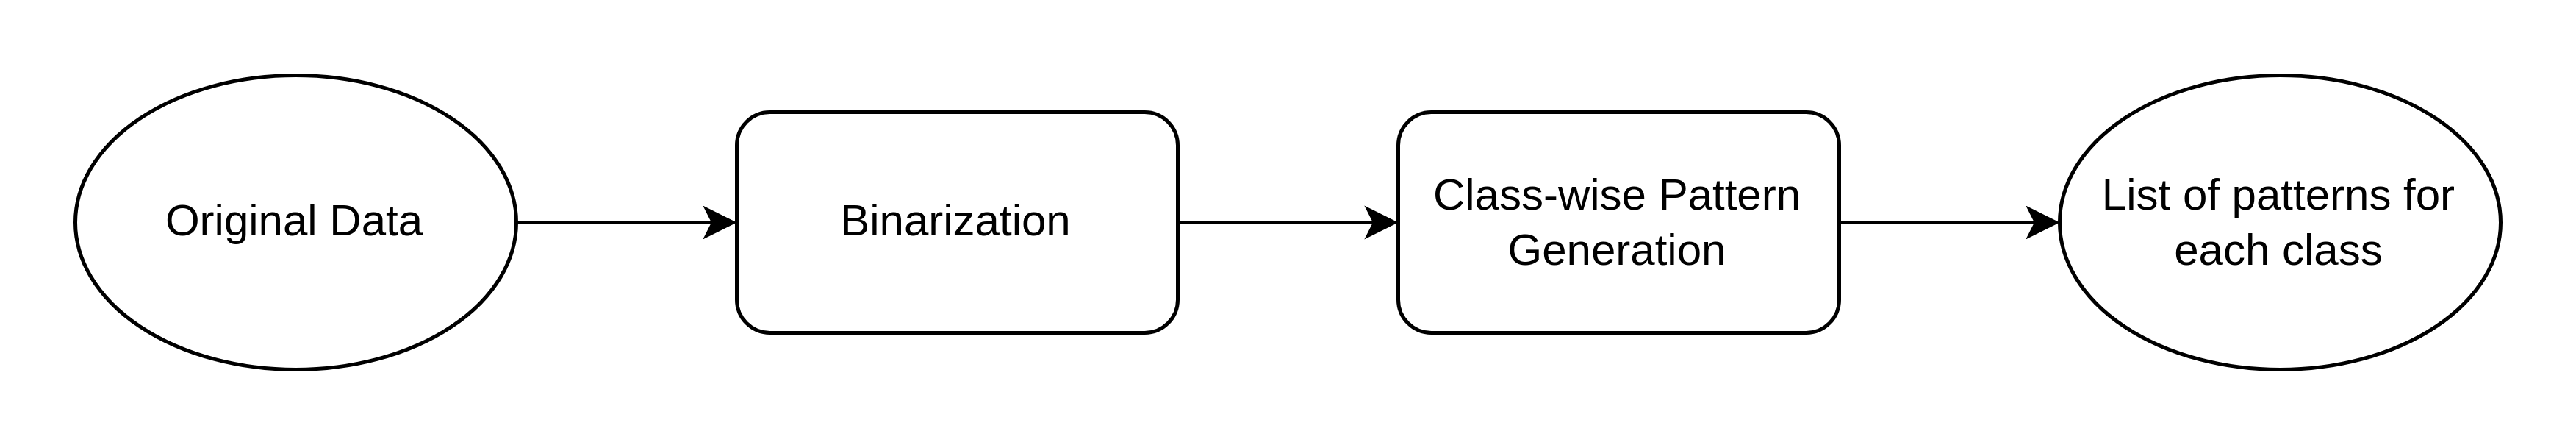
\includegraphics[width=\linewidth]{Methedology.drawio.png}
    \caption{LAD Process Flow}
    \label{fig:LAD}
\end{figure}

The main issue with most IDS systems is that they are resource intensive and logically ambiguous.

The proposed work is a modification of LAD which revolves around transforming data into binary format and generating rules in a Sum of Product format for the purpose of classification. The overall flow of the process is in stages: 

\begin{itemize}
    \item \textbf{Binarization:} Converting the data to binary format.
    \item \textbf{Pattern Generation:} Using binary data to make rules.
\end{itemize}


\subsection{Binarization}

\begin{figure}[ht!]
    \centering
    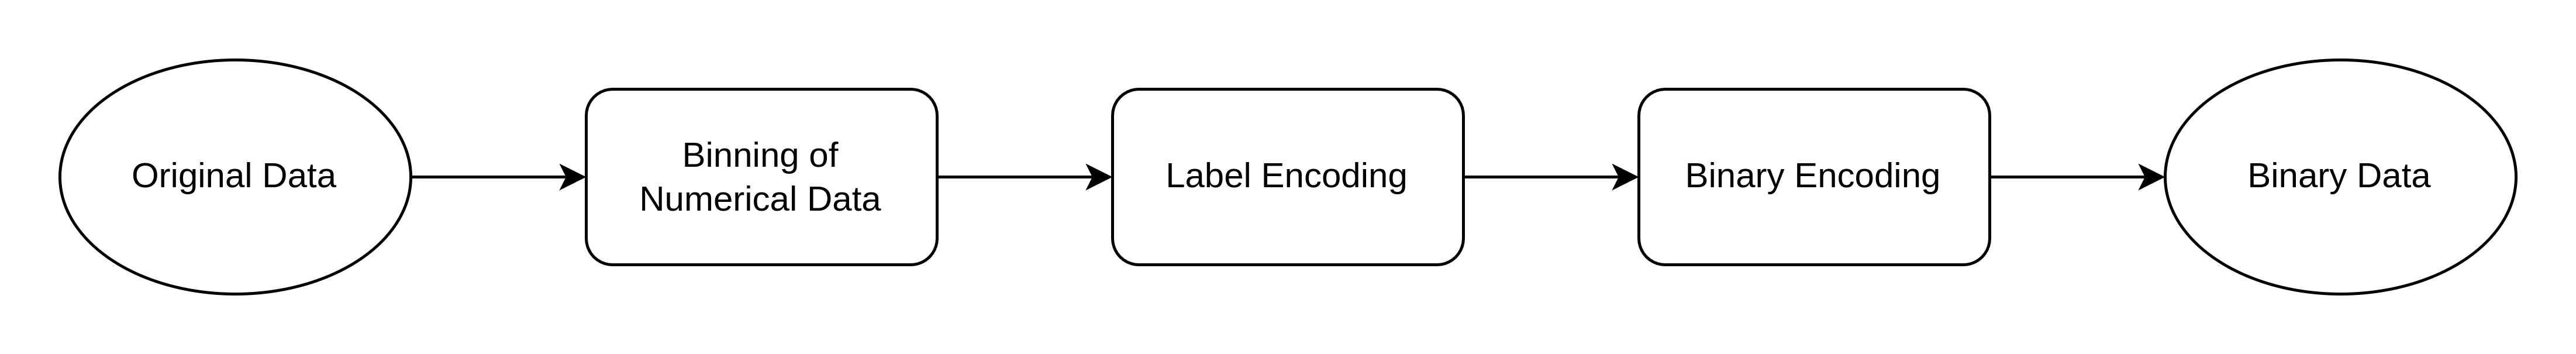
\includegraphics[width=\linewidth]{Binarization.drawio.png}
    \caption{Binarization Process}
    \label{fig:Binarization}
\end{figure}

The binarization process that transforms every feature in the dataset into one or more binary features.
This is done while aiming to encapsulate all the significant information present in them.
All features in the dataset are binarized independently.
Binarizing a numerical feature as is may produce too many binary features with minimum significance due to number of unique values being comparable to number of samples.
So, many of these values should be collected into groups which is done by the process called binning.

\begin{figure}[ht!]
    \centering
    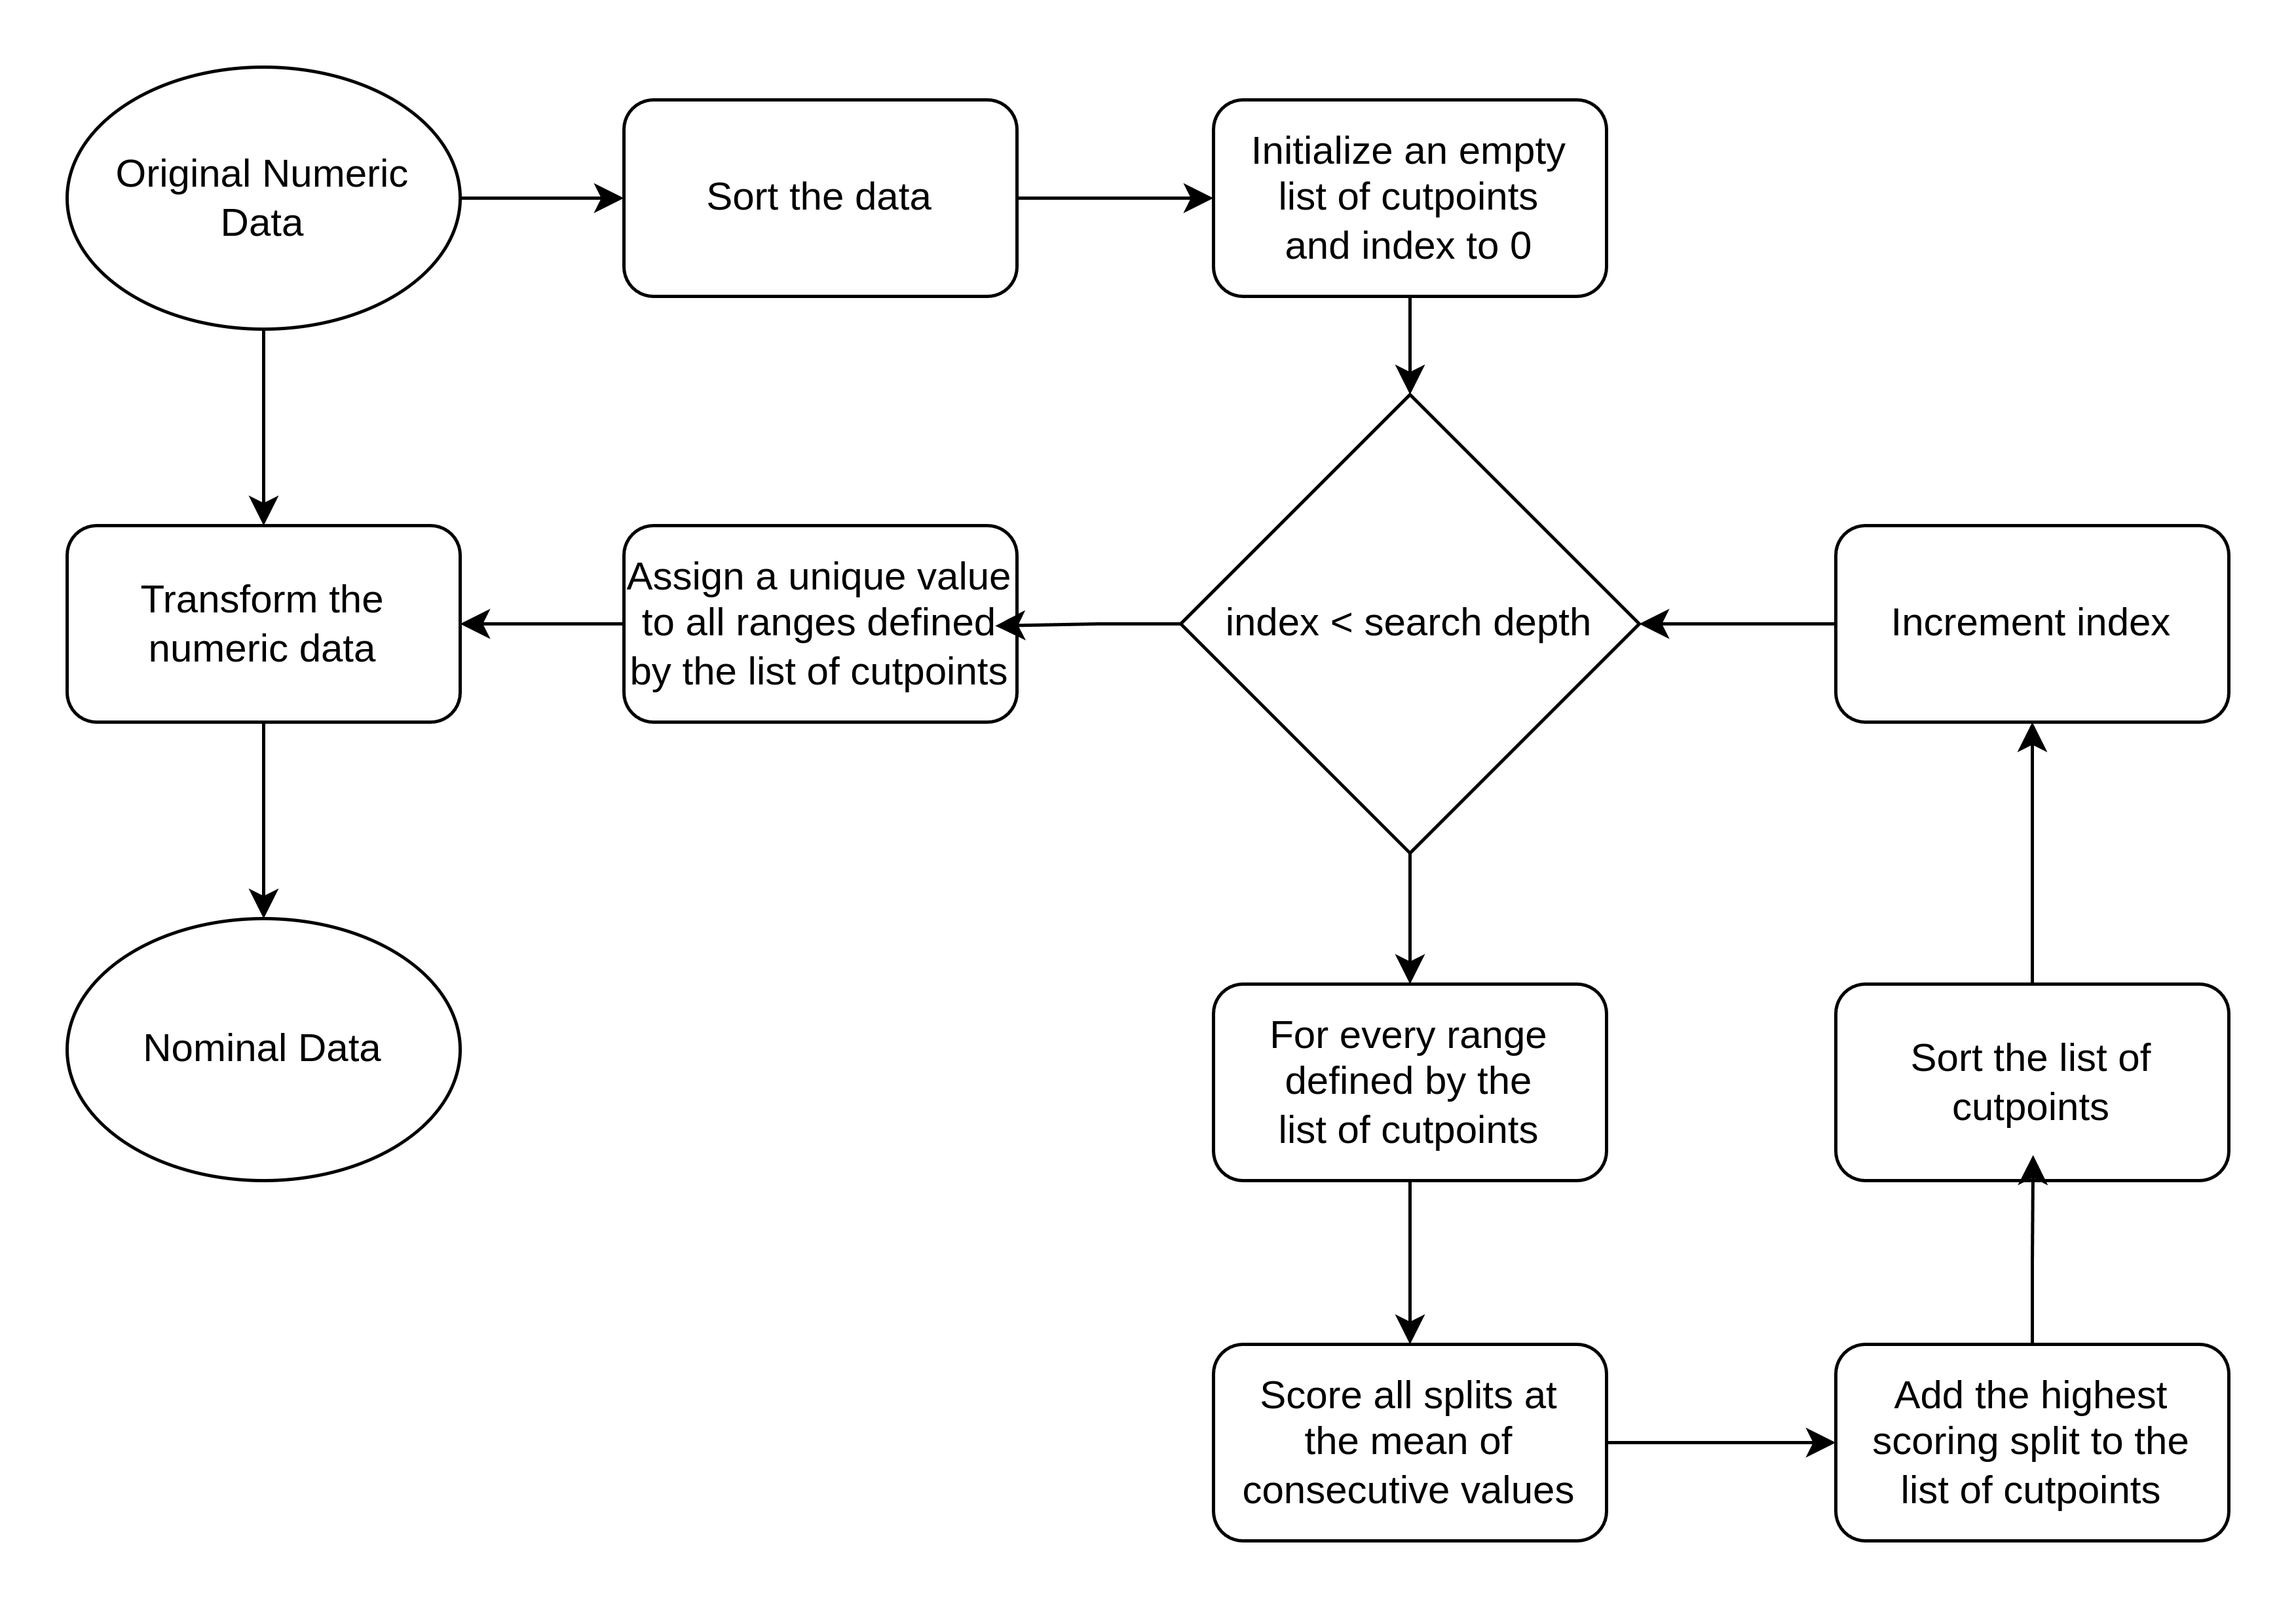
\includegraphics[width=0.5\linewidth]{Binning.drawio.png}
    \caption{Binning Process}
    \label{fig:Binning}
\end{figure}

In binning we transform continuous numerical data into various intervals.
This process begins with sorting of the data.
Then the arithmetic mean of all consecutive values is taken into consideration to obtain a cutpoint.
These values are then scored with the formula:
\[
\text{score} = \sqrt{\frac{\sum_{i=0}^{n-1} \sum_{j=i+1}^{n-1} (\text{rates}_i - \text{rates}_j)^2}{\frac{n^2 - (n \bmod 2)}{4}}}
\]
\begin{center}
\footnotesize{Where \(n\) is the number of classes, \(\text{rates}_i\) is the ratio of number of samples of class \(i\) that has appeared before the cutpoint to total number of samples in class \(i\).}
\end{center}

The value with the highest score if higher than a minimum threshold is stored as a cutpoint and used to divide the data into two.
The same process is repeated for both divisions of data to divide them further until either the highest score from all divisions is less than the threshold or a maximum depth of search is reached.

\begin{table}[ht!]
    \centering
    % \caption{Binning Example}

    \begin{talltblr}[
    caption = {Binning Example},
    label = {tab:binning_example}
    ]{columns = {c}, colspec={XX}}
    % First Row of Subtables
    \begin{tblr}{columns = {c}, column{1}={l}, vlines={2-Z}{solid}, hline{2,3,Z}, cell{1}{1} = {c=4}{c}}
        Original Sorted Values & & & \\
        \textbf{y} & \textbf{f4}  & \textbf{Cutpoint} & \textbf{Score} \\ 
         b &  7 & -    & -    \\
         b & 14 & 10.5 & 0.333\\
         a & 20 & 17   & 0.667\\
         b & 20 & -    & -    \\
         a & 22 & 21   & 0.75 \\
         a & 29 & 25.5 & 0.5  \\
         a & 31 & 30   & 0.25 \\
    \end{tblr} 
    &
    \begin{tblr}{columns = {c}, column{1}={l}, vlines={2-Z}{solid}, hline{2,3,Z}, cell{1}{1} = {c=4}{c}}
        Values after 1 Split \\
        \textbf{y} & \textbf{f4}  & \textbf{Cutpoint} & \textbf{Score} \\
         b &  7 & -    & -    \\
         b & 14 & 10.5 & 0.333\\
         a & 20 & 17   & 0.667\\
         b & 20 & -    & -    \\ \hline \hline
         a & 22 & -    & -    \\
         a & 29 & 25.5 & NaN  \\
         a & 31 & 30   & NaN  \\
    \end{tblr} 
    \\ % End of First Row
    % Second Row of Subtables
    \begin{tblr}{columns = {c}, column{1}={l}, vlines={2-Z}{solid}, hline{2,3,Z}, cell{1}{1} = {c=4}{c}}
        Values after 2 Split \\
        \textbf{y} & \textbf{f4}  & \textbf{Cutpoint} & \textbf{Score} \\
         b &  7 & -    & -  \\
         b & 14 & 10.5 & NaN\\ \hline \hline
         a & 20 & -    & -  \\
         b & 20 & -    & -  \\ \hline \hline
         a & 22 & -    & -  \\
         a & 29 & 25.5 & NaN\\
         a & 31 & 30   & NaN\\
    \end{tblr} 
    &
    \begin{tblr}{columns = {c}, column{1}={l}, vlines={2-Z}{solid}, hline{2,3,Z}, cell{1}{1} = {c=3}{c}}
        Binning of Numerical Data \\
        \textbf{y} & \textbf{f4} & \textbf{f4 ranges} \\
         a & 31& \((21, \infty)\)  \\
         a & 29& \((21, \infty)\)  \\
         a & 20& \((17, 21)\)      \\
         a & 22& \((21, \infty)\)  \\
         b & 20& \((17, 21)\)      \\
         b & 14& \((-\infty, 17)\) \\
         b &  7& \((-\infty, 17)\) \\
    \end{tblr} 
    \\ % End of Second Row
    \end{talltblr}

    % \label{tab:binning_example}
\end{table}

All selected cutpoints are collectively used to make ranges by sorting them in ascending order along with \(-\infty\) and \(\infty\).
Consecutive values are used as boundaries of ranges which form the bins that all collectively ideally represent the original data in discrete or nominal form.

Every unique value in nominal features or bin created from numerical features are assigned a unique numerical value for said feature.
These numerical value are processed as their binary form, using every bit of those values for a distinct binary feature.
This process is repeated for every feature thereby binarizing all the data.

\begin{table}[ht!]
    \centering
    % \label{tab:binarization}
    \begin{talltblr}[
    caption = {Binarization Example},
    label = {tab:binarization}
    ]{columns = {c}, cell{2}{1} = {c = 2}{c}, cell{3}{1} = {c = 2}{c}, colspec={XX}}   % First Row of Subtables
    \begin{tblr}{columns = {c}, column{1} = {l}, cell{1}{1} = {c = 5}{c}, vlines = {2-Z}{solid}, hline{2,3,Z}}
      Original Values \\ 
        \textbf{y} & \textbf{f1} & \textbf{f2}  & \textbf{f3} & \textbf{f4} \\
         a &  1 & green & yes & 31 \\
         a &  4 & blue  & no  & 29 \\
         a &  2 & blue  & yes & 20 \\
         a &  4 & red   & no  & 22 \\
         b &  3 & red   & yes & 20 \\
         b &  2 & green & no  & 14 \\
         b &  4 & green & no  & 7  \\ 
    \end{tblr}
    &
\begin{tblr}{columns = {c}, column{1} = {l}, cell{1}{1} = {c = 5}{c}, vlines = {2-Z}{solid}, hline{2,3,Z}}
  Binning of Numerical Data \\
  \textbf{y} & \textbf{f1} & \textbf{f2}  & \textbf{f3} & \textbf{f4}  \\
   a &  \((-\infty, 1.5)\) & green & yes & \((21, \infty)\) \\
   a &  \((3.5, \infty)\) & blue  & no  & \((21, \infty)\) \\
   a &  \((1.5, 2.5)\)   & blue  & yes & \((17, 21)\)     \\
   a &  \((3.5, \infty)\) & red   & no  & \((21, \infty)\) \\
   b &  \((2.5, 3.5)\)   & red   & yes & \((17, 21)\)     \\
   b &  \((1.5, 2.5)\)   & green & no  & \((-\infty, 17)\) \\
   b &  \((3.5, \infty)\) & green & no  & \((-\infty, 17)\) \\
\end{tblr}
    \\
    % Second Row of Subtables

\begin{tblr}{columns = {c}, column{1} = {l}, cell{1}{1} = {c = 5}{c}, vlines = {2-Z}{solid}, hline{2,3,Z}}
  Label Encoding \\
  \textbf{y} & \textbf{f1} & \textbf{f2}  & \textbf{f3} & \textbf{f4} \\
   a & 0 & 0 & 1 & 2 \\
   a & 3 & 1 & 0 & 2 \\
   a & 1 & 1 & 1 & 1 \\
   a & 3 & 2 & 0 & 2 \\
   b & 2 & 2 & 1 & 1 \\
   b & 1 & 0 & 0 & 0 \\
   b & 3 & 0 & 0 & 0 \\ 
\end{tblr}
    \\
\begin{tblr}{columns = {c}, column{1} = {l}, cell{1}{1} = {c = 8}{c}, vlines = {2-Z}{solid}, hline{2,3,Z}}
  Binarized Values \\
  \textbf{y} & \textbf{b1\_1} & \textbf{b1\_0} & \textbf{b2\_1} & \textbf{b2\_0} & \textbf{b3} & \textbf{b4\_1} & \textbf{b4\_0} \\
   a & false & false & false & false & true  & true  & false \\
   a & true  & true  & false & true  & false & true  & false \\
   a & false & true  & false & true  & true  & false & true  \\
   a & true  & true  & true  & false & false & true  & false \\
   b & true  & false & true  & false & true  & false & true  \\
   b & false & true  & false & false & false & false & false \\
   b & true  & true  & false & false & false & false & false \\
\end{tblr}
    \end{talltblr}

\end{table}


Table \ref{tab:binarization} demonstrates how original feature values are sequentially transformed through the steps of binning, label encoding, and binary conversion, highlighting the systematic nature of the binarization process and its effectiveness in preparing data for further analysis.

\subsection{Pattern Generation}

Once the data is binarized, patterns are generated for the purpose of classification.
Firstly, an empty list of rules and list of patterns that contains a single blank pattern is generated as a starting point.

\begin{figure}[ht!]
    \centering
    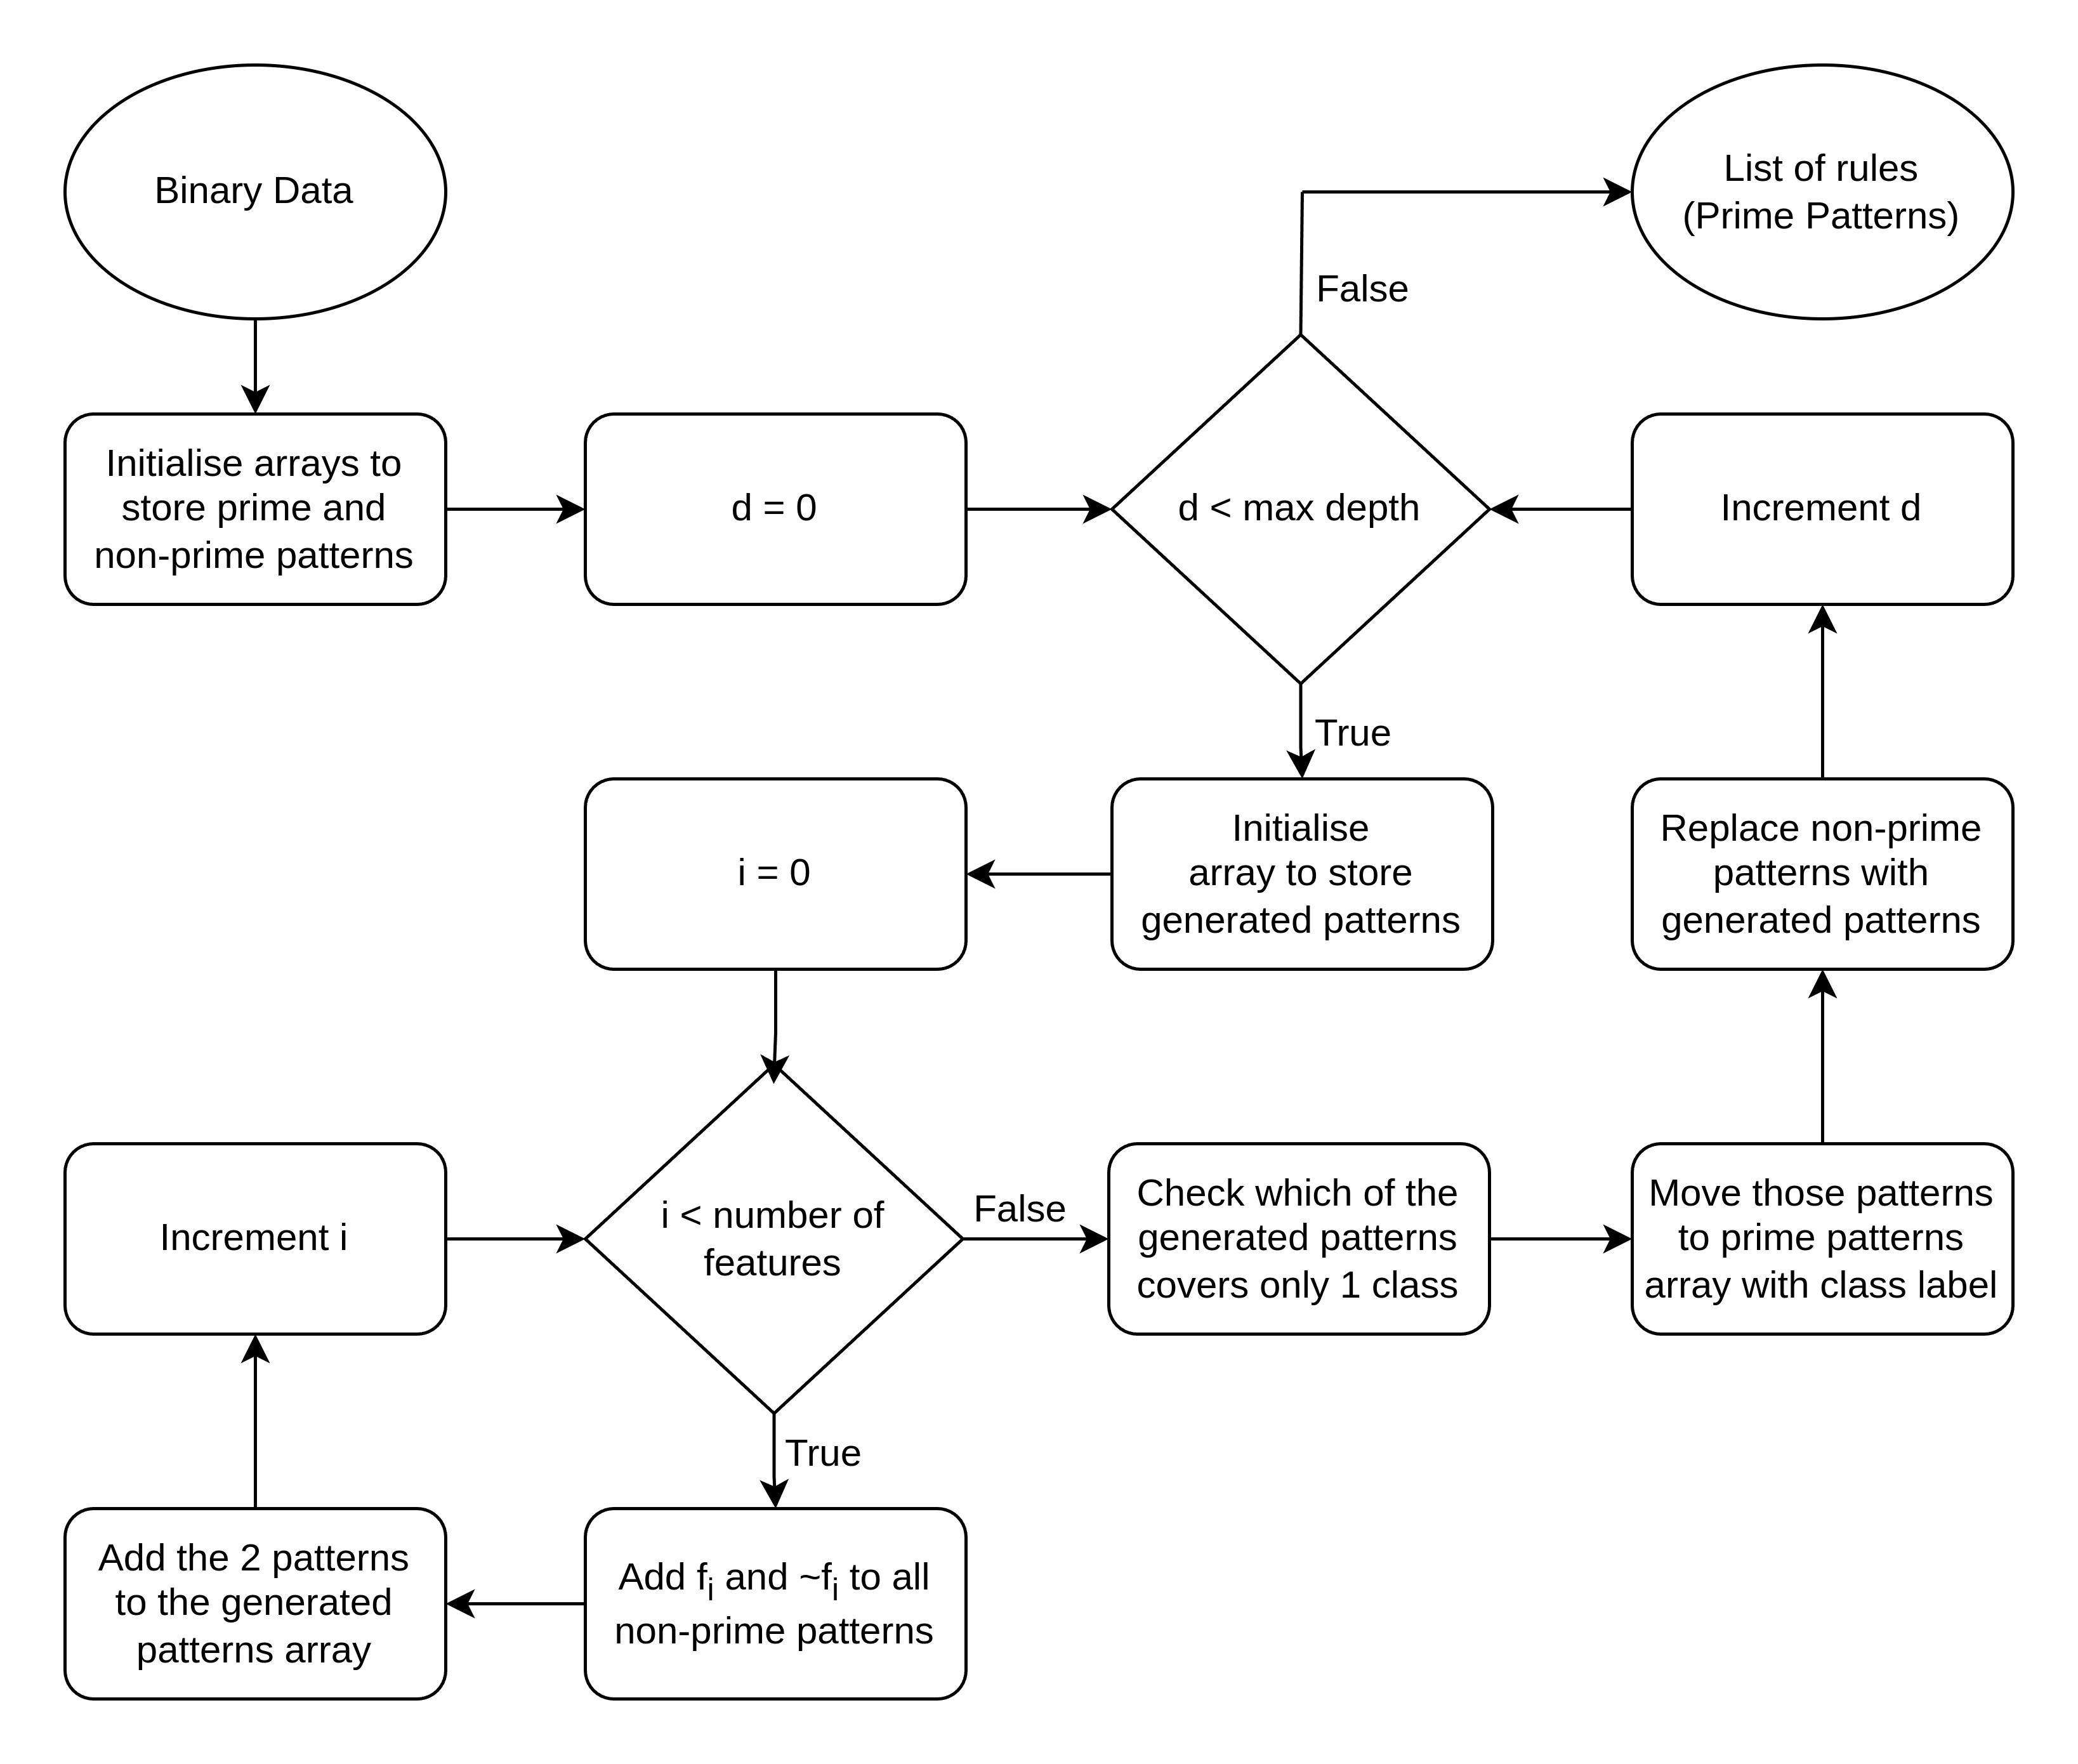
\includegraphics[width=0.8\linewidth]{Pattern.drawio.png}
    \caption{Pattern Generation Process}
    \label{fig:PatternGeneration}
\end{figure}

Following this, from each existing pattern two new pattern for every feature in binary data are generated by adding each feature once as is and once as its inverse to the pattern.
Next, patterns that specifically cover instances of a single class are identified and moved to the list of rules with the association with said class.
The observations that are covered by these rules are removed from consideration for new rules.
The patterns that do not cover a single class are retained for further iterations.
This process is repeated until either all data points are covered by the generated rules or a predefined maximum number of iterations is reached.

\subsection{Classification}
For classification of each sample a short circuiting approach is used.
The evaluation is done by matching the sample to every rule in the order the rules were generated.
Which stops as soon as a matching rule is found and the sample is classified with the class associated with that rule.
If no rules match the sample, its class is set to NULL.


\section{Results and Analysis}\label{sec:Results}
This section presents the results of our experiments evaluating the proposed intrusion detection method using the NSLKDD and KDDCup99 (10\%) datasets.
% We analyze performance metrics, rule generation, and decision matrices to assess the model's effectiveness.
Additionally, we discuss the limitations of the approach.


\subsection{System Configuration}

The experiments and analyses were conducted on a high-performance HP Z640 Workstation equipped with an Intel Xeon E5-2620 v3 processor (12 cores, 3.20 GHz), 15.52 GiB of RAM, and an NVIDIA Quadro K2200 GPU. The system ran Fedora Linux 41 (Workstation Edition) x86\_64, with the Linux 6.11.8-300.fc41.x86\_64 kernel, utilizing the COSMIC 1.0.0~alpha.3\_20241120-1.fc41 desktop environment and the Wayland-based \texttt{cosmic-comp} window manager.
The algorithm was implemented in Rust 1.82.0 using the polars crate which was interfaced with python using the crate pyo3. Python was used to load and run datasets using the polars library.

\subsection{Dataset Description}
We utilize two popular intrusion detection datasets, as shown in Table~\ref{tab:dataset}.
\begin{table}[ht!]
    \centering
    \caption{Datasets}
    \begin{tabular}{|l|r|c|c|}
        \hline
        \textbf{Dataset} & \textbf{Samples} & \textbf{Features} & \textbf{Classes} \\
        \hline
        NSL-KDD \cite{DATA1} & 125,973 & 41 & 23 \\
        \hline
        KDD-Cup99 \cite{DATA2}  & 4,898,431 & 41 & 23 \\
        \hline
    \end{tabular}
    \label{tab:dataset}
\end{table}
These datasets contain labeled network traffic data, representing normal and malicious activities.

\subsection{Performance Metrics}
The following performance metrics were used to evaluate the results:

\begin{itemize} 
    \item \textbf{Accuracy}: The proportion of correctly predicted instances out of the total instances.
    \[
    \text{Accuracy} = \frac{TP + TN}{TP + TN + FP + FN}
    \]
    \item \textbf{Precision}: The ratio of true positive predictions to the total predicted positives (i.e., how many selected items were relevant).
    \[
    \text{Precision} = \frac{TP}{TP+FP}
    \]
    \item \textbf{Recall}: The ratio of true positives to the actual positives in the dataset (i.e., how many relevant items were selected).
    \[
    \text{Recall} = \frac{TP}{TP+FN}
    \]
    \item \textbf{F2-Score}: A weighted harmonic mean of precision and recall that gives more importance to recall, calculated as:
    \[
    \text{F2-Score} = \frac{5 \cdot \text{Precision} \cdot \text{Recall}}{4 \cdot \text{Precision} + \text{Recall}}.
    \]
    \item \textbf{Data Coverage}: The proportion of predicted instances out of the total instances.
\end{itemize}

\subsection{Tabular Results}
The results presented in this section pertain to experiments conducted with a maximum depth of 4 for pattern generation.
Table~\ref{tab:4result} provides an overview of the performance metrics across the datasets NSLKDD and KDDCup99 (10\%).
The metrics include accuracy, precision, recall, F2-score, and coverage.
For the NSLKDD dataset, the accuracy achieved was 75.48\%, with a precision of 85.58\%, a recall of 75.48\%, an F2-score of 77.30\%, and a coverage of 92.56\%.
On the other hand, the KDDCup99 (10\%) dataset exhibited significantly higher performance with an accuracy of 96.10\%, a precision of 99.96\%, a recall of 96.10\%, an F2-score of 96.85\%, and a coverage of 96.13\%.
These results demonstrate the effectiveness of the proposed method, particularly for the KDDCup99 dataset.

\begin{table}[ht!]
    \centering
    \caption{Performance Metrics for Different Datasets}
    \begin{tabular}{lccccc}
    \toprule
    \textbf{Dataset} & \textbf{Accuracy} & \textbf{Precision} & \textbf{Recall} & \textbf{F2-Score} & \textbf{Coverage} \\
    \midrule
    NSLKDD & 75.48\% & 85.58\% & 75.48\% & 77.30\% & 92.56\% \\
    KDDCup99 (10\%) & 96.10\% & 99.96\% & 96.10\% & 96.85\% & 96.13\% \\
    \bottomrule
    \end{tabular}
    \label{tab:4result}
\end{table}

Table~\ref{tab:Dataset_Samples} provides insights into the characteristics of the datasets used in the experiments.
The KDDCup99 (10\%) dataset consists of 330,994 samples with 41 features, 32 of which are preprocessed and 29 are binarized.
In contrast, the NSLKDD dataset comprises 125,973 samples with 41 features, of which 54 are binarized.
These details emphasize the variability in dataset size and feature representation, highlighting the adaptability of the binarization and rule-generation process.

\begin{table}[ht!]
    \centering
    \caption{Dataset Samples and Features}
    \begin{tabular}{lcc}
    \toprule
    \textbf{Dataset} & \textbf{Samples} & \textbf{Features} \\
    \midrule
    KDDCup99 (10\%) & 330,994 & 41 (32 preprocessed, 29 binarized) \\
    NSLKDD & 125,973 & 41 (54 binarized) \\
    \bottomrule
    \end{tabular}
    \label{tab:Dataset_Samples}
\end{table}

Table~\ref{tab:Rules_Generated} focuses on the number of rules generated for the datasets based on different minimum match criteria at a depth of 3.
For the KDDCup99 dataset, 243 rules were generated for at least one match, 85 for a minimum of 10 matches, and 42 for a minimum of 50 matches.
Similarly, for the NSLKDD dataset, the number of rules generated was 365, 150, and 65 for minimum matches of 1, 10, and 50, respectively.
These statistics indicate how stricter matching criteria reduce the number of generated rules, ensuring more selective and meaningful rules.

\begin{table}[ht!]
    \centering
    \caption{Number of Rules Generated for Different Minimum Matches of Sample at depth 3}
    \begin{tabular}{lcc}
    \toprule
    \textbf{Matches} & \textbf{KDDCup99 (10\%)} & \textbf{NSLKDD} \\
    \midrule
    1 & 243 & 365 \\
    10 & 85 & 150 \\
    50 & 42 & 65 \\
    \bottomrule
    \end{tabular}
    \label{tab:Rules_Generated}
\end{table}

Table~\ref{tab:Overall_Metrics} summarizes the overall metrics for both datasets under different matching criteria. 
For the KDDCup99 dataset, with at least one match, the accuracy, precision, recall, and coverage were 95.91\%, 99.96\%, 95.91\%, and 95.94\%, respectively. As the match criteria increased to 10 and 50, the accuracy and recall reduced to 93.27\% and 75.80\%, respectively, but the precision remained extremely high (99.98\% and 99.97\%). Similarly, for the NSLKDD dataset, stricter match criteria also led to lower accuracy and recall while maintaining high precision. For instance, at one match, the accuracy was 75.42\%, which dropped to 71.93\% and 70.08\% for match criteria of 10 and 50, respectively.

\begin{table}[ht!]
    \centering
    \caption{Overall Metrics for Different Matching Criteria}
    \begin{tabular}{lcccccc}
    \toprule
    \textbf{Dataset} & \textbf{Matches} & \textbf{Acc} & \textbf{Prec} & \textbf{Recall} & \textbf{F2-Score} & \textbf{Coverage} \\
    \midrule
    \multirow{3}{*}{KDDCup99} & 1 & 95.91\% & 99.96\% & 95.91\% & - & 95.94\% \\
    & 10 & 93.27\% & 99.98\% & 93.27\% & - & 93.29\% \\
    & 50 & 75.80\% & 99.97\% & 75.80\% & - & 75.81\% \\
    \midrule
    \multirow{3}{*}{NSLKDD} & 1 & 75.42\% & 86.13\% & 75.42\% & - & 91.52\% \\
    & 10 & 71.93\% & 87.29\% & 71.93\% & - & 85.55\% \\
    & 50 & 70.08\% & 88.83\% & 70.08\% & - & 81.17\%\\
    \bottomrule
    \end{tabular}
    \label{tab:Overall_Metrics}
\end{table}

The decision matrices provided in Tables~\ref{tab:NSLKDD_Matrix} and \ref{tab:KDDcup_Matrix} offer a detailed view of classification performance for the NSLKDD and KDDCup99 datasets under varying minimum match criteria.
For the NSLKDD dataset, as shown in Table~\ref{tab:NSLKDD_Matrix}, the number of correctly classified "Attack" and "Normal" instances decreases as the minimum match criterion becomes stricter, resulting in an increase in \textit{NULL} (unmatched) cases.
For instance, with a minimum of one match, there were 8,295 correctly classified "Attack" instances and 8,709 "Normal" instances. However, with a minimum of 50 matches, these numbers reduced to 7,725 and 8,073, respectively.
A similar trend is observed in the decision matrices for the KDDCup99 dataset in Table~\ref{tab:KDDcup_Matrix}. For example, with one match, 124,431 "DOS" instances and 30,515 "Normal" instances were correctly classified, while with 50 matches, these numbers dropped to 95,373 and 27,265, respectively.
This illustrates the trade-off between stricter match criteria and classification coverage.

\begin{table}[ht!]
    \centering
    \caption{Decision Matrix for NSLKDD}
    \label{tab:NSLKDD_Matrix}

    \begin{tabular}{c}

    % Subtable 1
    \begin{tabular}{|l|c|c|r|}
        \hline
        \multicolumn{4}{|c|}{\textbf{For Minimum 1 Matching Sample}} \\ \hline
         & \textbf{Attack} & \textbf{Normal} & \textit{NULL} \\  \hline 
        \textbf{Attack} & 8295 & 3336 & 1202 \\ \hline 
        \textbf{Normal} & 292 & 8709 & 710 \\ \hline
    \end{tabular}

\\
\\
    % Subtable 2
    \begin{tabular}{|l|c|c|r|}
        \hline
        \multicolumn{4}{|c|}{\textbf{For Minimum 10 Matching Samples}} \\ \hline
         & \textbf{Attack} & \textbf{Normal} & \textit{NULL} \\  \hline 
        \textbf{Attack} & 7781 & 2801 & 2151 \\ \hline 
        \textbf{Normal} & 268 & 8336 & 1107 \\ \hline
    \end{tabular}

\\
\\
    % Subtable 3
    \begin{tabular}{|l|c|c|r|}
        \hline
        \multicolumn{4}{|c|}{\textbf{For Minimum 50 Matching Samples}} \\ \hline
         & \textbf{Attack} & \textbf{Normal} & \textit{NULL} \\  \hline 
        \textbf{Attack} & 7725 & 2253 & 2855 \\ \hline 
        \textbf{Normal} & 247 & 8073 & 1391 \\ \hline
    \end{tabular}

    \end{tabular}

\end{table}

\begin{table}[ht!]
    \centering
    \caption{Decision Matrix for KDDCup (10\%)}
    \label{tab:KDDcup_Matrix}

    \begin{tabular}{c}

    % Subtable 1
    \begin{tabular}{|l|c|c|c|c|c|r|}
        \hline
        \multicolumn{7}{|c|}{\textbf{For Minimum 1 Matching Sample}} \\ \hline
         & \textbf{DOS} & \textbf{Normal} & \textbf{Probe} & \textbf{R2L} & \textbf{U2R} & \textit{NULL} \\ \hline 
        \textbf{DOS} & 124431 & 8 & 0 & 0 & 0 & 4742 \\ \hline 
        \textbf{Normal} & 3 & 30515 & 3 & 2 & 5 & 1574 \\ \hline
        \textbf{Probe} & 2 & 8 & 1259 & 0 & 0 & 86 \\ \hline
        \textbf{R2L} & 0 & 10 & 0 & 42 & 1 & 219 \\ \hline
        \textbf{U2R} & 1 & 1 & 0 & 2 & 13 & 0 \\ \hline
    \end{tabular}

\\
\\
    % Subtable 2
    \begin{tabular}{|l|c|c|c|c|c|r|}
        \hline
        \multicolumn{7}{|c|}{\textbf{For Minimum 10 Matching Samples}} \\ \hline
         & \textbf{DOS} & \textbf{Normal} & \textbf{Probe} & \textbf{R2L} & \textbf{U2R} & \textit{NULL} \\ \hline 
        \textbf{DOS} & 123506 & 4 & 0 & 0 & 0 & 5671 \\ \hline 
        \textbf{Normal} & 1 & 27529 & 1 & 1 & 0 & 4570 \\ \hline
        \textbf{Probe} & 1 & 2 & 898 & 0 & 0 & 454 \\ \hline
        \textbf{R2L} & 0 & 8 & 0 & 123 & 0 & 241 \\ \hline
        \textbf{U2R} & 1 & 2 & 0 & 1 & 7 & 6 \\ \hline
    \end{tabular}

\\
\\
    % Subtable 3
    \begin{tabular}{|l|c|c|c|c|c|r|}
        \hline
        \multicolumn{7}{|c|}{\textbf{For Minimum 50 Matching Samples}} \\ \hline
         & \textbf{DOS} & \textbf{Normal} & \textbf{Probe} & \textbf{R2L} & \textbf{U2R} & \textit{NULL} \\ \hline 
        \textbf{DOS} & 95373 & 3 & 0 & 0 & 0 & 33805 \\ \hline 
        \textbf{Normal} & 1 & 27265 & 2 & 1 & 0 & 4833 \\ \hline
        \textbf{Probe} & 4 & 2 & 843 & 0 & 0 & 504 \\ \hline
        \textbf{R2L} & 0 & 4 & 0 & 94 & 0 & 274 \\ \hline
        \textbf{U2R} & 1 & 2 & 0 & 0 & 0 & 14 \\ \hline
    \end{tabular}

    \end{tabular}
\end{table}

Overall, the tables provide a comprehensive view of the performance and effectiveness of the binarization and rule-generation framework across multiple datasets, emphasizing how various factors, such as dataset characteristics and matching criteria, influence the classification results.


\subsection{Limitations of Proposed Work}
The proposed method has some limitations:

\begin{itemize}
    \item \textbf{Long Training Time:} The training time of LAD is of the order \( O(scf^d) \), where \(s\) is the number of samples, \(c\) is the number of classes, \(f\) is the number of features in the binarized data, and \(d\) is the maximum number of attributes in a rule.
    \item \textbf{Incomplete Coverage of Dataset:} The dataset may not be completely covered by LAD if the maximum number of attributes is not set to a sufficiently high value.
\end{itemize}

\section{Conclusion} \label{sec:Conclusion}

In this study, we explored the application of a Learning Algorithm for Intrusion Detection (LAD) on two well-known intrusion detection datasets: NSL-KDD and KDD-Cup99. The experiments were conducted on a high-performance workstation, and various performance metrics, including accuracy, precision, recall, F2-score, and data coverage, were used to evaluate the effectiveness of the proposed method. 

The results indicated that LAD achieved a good balance between performance and data coverage across both datasets. Specifically, the method demonstrated high accuracy and precision, especially on the KDD-Cup99 dataset (10\% subset), with an accuracy of 96.10\% and precision of 99.96\%. However, it was also observed that LAD exhibited limitations, such as long training times and incomplete dataset coverage when the maximum number of attributes was not sufficiently set.

Despite these challenges, the proposed approach provided valuable insights into improving the effectiveness of intrusion detection systems, and future work may focus on addressing the limitations related to training time and dataset coverage to enhance the overall performance of the system. 

In conclusion, the findings from this study contribute to the development of more efficient and accurate intrusion detection techniques, with potential for further optimization in future research.



% \section{Results}\label{sec2}

% Sample body text. Sample body text. Sample body text. Sample body text. Sample body text. Sample body text. Sample body text. Sample body text.

% \section{This is an example for first level head---section head}\label{sec3}

% \subsection{This is an example for second level head---subsection head}\label{subsec2}

% \subsubsection{This is an example for third level head---subsubsection head}\label{subsubsec2}

% Sample body text. Sample body text. Sample body text. Sample body text. Sample body text. Sample body text. Sample body text. Sample body text. 

% \section{Equations}\label{sec4}

% Equations in \LaTeX\ can either be inline or on-a-line by itself (``display equations''). For
% inline equations use the \verb+$...$+ commands. E.g.: The equation
% $H\psi = E \psi$ is written via the command \verb+$H \psi = E \psi$+.

% For display equations (with auto generated equation numbers)
% one can use the equation or align environments:
% \begin{equation}
% \|\tilde{X}(k)\|^2 \leq\frac{\sum\limits_{i=1}^{p}\left\|\tilde{Y}_i(k)\right\|^2+\sum\limits_{j=1}^{q}\left\|\tilde{Z}_j(k)\right\|^2 }{p+q}.\label{eq1}
% \end{equation}
% where,
% \begin{align}
% D_\mu &=  \partial_\mu - ig \frac{\lambda^a}{2} A^a_\mu \nonumber \\
% F^a_{\mu\nu} &= \partial_\mu A^a_\nu - \partial_\nu A^a_\mu + g f^{abc} A^b_\mu A^a_\nu \label{eq2}
% \end{align}
% Notice the use of \verb+\nonumber+ in the align environment at the end
% of each line, except the last, so as not to produce equation numbers on
% lines where no equation numbers are required. The \verb+\label{}+ command
% should only be used at the last line of an align environment where
% \verb+\nonumber+ is not used.
% \begin{equation}
% Y_\infty = \left( \frac{m}{\textrm{GeV}} \right)^{-3}
%     \left[ 1 + \frac{3 \ln(m/\textrm{GeV})}{15}
%     + \frac{\ln(c_2/5)}{15} \right]
% \end{equation}
% The class file also supports the use of \verb+\mathbb{}+, \verb+\mathscr{}+ and
% \verb+\mathcal{}+ commands. As such \verb+\mathbb{R}+, \verb+\mathscr{R}+
% and \verb+\mathcal{R}+ produces $\mathbb{R}$, $\mathscr{R}$ and $\mathcal{R}$
% respectively (refer Subsubsection~\ref{subsubsec2}).

% \section{Tables}\label{sec5}

% Tables can be inserted via the normal table and tabular environment. To put
% footnotes inside tables you should use \verb+\footnotetext[]{...}+ tag.
% The footnote appears just below the table itself (refer Tables~\ref{tab1} and \ref{tab2}). 
% For the corresponding footnotemark use \verb+\footnotemark[...]+

% \begin{table}[ht!]
% \caption{Caption text}\label{tab1}%
% \begin{tabular}{@{}llll@{}}
% \toprule
% Column 1 & Column 2  & Column 3 & Column 4\\
% \midrule
% row 1    & data 1   & data 2  & data 3  \\
% row 2    & data 4   & data 5\footnotemark[1]  & data 6  \\
% row 3    & data 7   & data 8  & data 9\footnotemark[2]  \\
% \botrule
% \end{tabular}
% \footnotetext{Source: This is an example of table footnote. This is an example of table footnote.}
% \footnotetext[1]{Example for a first table footnote. This is an example of table footnote.}
% \footnotetext[2]{Example for a second table footnote. This is an example of table footnote.}
% \end{table}

% \noindent
% The input format for the above table is as follows:

% %%=============================================%%
% %% For presentation purpose, we have included  %%
% %% \bigskip command. Please ignore this.       %%
% %%=============================================%%
% \bigskip
% \begin{verbatim}
% \begin{table}[<placement-specifier>]
% \caption{<table-caption>}\label{<table-label>}%
% \begin{tabular}{@{}llll@{}}
% \toprule
% Column 1 & Column 2 & Column 3 & Column 4\\
% \midrule
% row 1 & data 1 & data 2	 & data 3 \\
% row 2 & data 4 & data 5\footnotemark[1] & data 6 \\
% row 3 & data 7 & data 8	 & data 9\footnotemark[2]\\
% \botrule
% \end{tabular}
% \footnotetext{Source: This is an example of table footnote. 
% This is an example of table footnote.}
% \footnotetext[1]{Example for a first table footnote.
% This is an example of table footnote.}
% \footnotetext[2]{Example for a second table footnote. 
% This is an example of table footnote.}
% \end{table}
% \end{verbatim}
% \bigskip
% %%=============================================%%
% %% For presentation purpose, we have included  %%
% %% \bigskip command. Please ignore this.       %%
% %%=============================================%%

% \begin{table}[ht!]
% \caption{Example of a lengthy table which is set to full textwidth}\label{tab2}
% \begin{tabular*}{\textwidth}{@{\extracolsep\fill}lcccccc}
% \toprule%
% & \multicolumn{3}{@{}c@{}}{Element 1\footnotemark[1]} & \multicolumn{3}{@{}c@{}}{Element 2\footnotemark[2]} \\\cmidrule{2-4}\cmidrule{5-7}%
% Project & Energy & $\sigma_{calc}$ & $\sigma_{expt}$ & Energy & $\sigma_{calc}$ & $\sigma_{expt}$ \\
% \midrule
% Element 3  & 990 A & 1168 & $1547\pm12$ & 780 A & 1166 & $1239\pm100$\\
% Element 4  & 500 A & 961  & $922\pm10$  & 900 A & 1268 & $1092\pm40$\\
% \botrule
% \end{tabular*}
% \footnotetext{Note: This is an example of table footnote. This is an example of table footnote this is an example of table footnote this is an example of~table footnote this is an example of table footnote.}
% \footnotetext[1]{Example for a first table footnote.}
% \footnotetext[2]{Example for a second table footnote.}
% \end{table}

% In case of double column layout, tables which do not fit in single column width should be set to full text width. For this, you need to use \verb+\begin{table*}+ \verb+...+ \verb+\end{table*}+ instead of \verb+\begin{table}+ \verb+...+ \verb+\end{table}+ environment. Lengthy tables which do not fit in textwidth should be set as rotated table. For this, you need to use \verb+\begin{sidewaystable}+ \verb+...+ \verb+\end{sidewaystable}+ instead of \verb+\begin{table*}+ \verb+...+ \verb+\end{table*}+ environment. This environment puts tables rotated to single column width. For tables rotated to double column width, use \verb+\begin{sidewaystable*}+ \verb+...+ \verb+\end{sidewaystable*}+.

% \begin{sidewaystable}[p]
% \caption{Tables which are too long to fit, should be written using the ``sidewaystable'' environment as shown here}\label{tab3}
% \begin{tabular*}{0.99\textheight}{@{\extracolsep\fill}lcccccc}
% \toprule%
% & \multicolumn{3}{@{}c@{}}{Element 1\footnotemark[1]}& \multicolumn{3}{@{}c@{}}{Element\footnotemark[2]} \\\cmidrule{2-4}\cmidrule{5-7}%
% Projectile & Energy	& $\sigma_{calc}$ & $\sigma_{expt}$ & Energy & $\sigma_{calc}$ & $\sigma_{expt}$ \\
% \midrule
% Element 3 & 990 A & 1168 & $1547\pm12$ & 780 A & 1166 & $1239\pm100$ \\
% Element 4 & 500 A & 961  & $922\pm10$  & 900 A & 1268 & $1092\pm40$ \\
% Element 5 & 990 A & 1168 & $1547\pm12$ & 780 A & 1166 & $1239\pm100$ \\
% Element 6 & 500 A & 961  & $922\pm10$  & 900 A & 1268 & $1092\pm40$ \\
% \botrule
% \end{tabular*}
% \footnotetext{Note: This is an example of table footnote this is an example of table footnote this is an example of table footnote this is an example of~table footnote this is an example of table footnote.}
% \footnotetext[1]{This is an example of table footnote.}
% \end{sidewaystable}

% \section{Figures}\label{sec6}

% As per the \LaTeX\ standards you need to use eps images for \LaTeX\ compilation and \verb+pdf/jpg/png+ images for \verb+PDFLaTeX+ compilation. This is one of the major difference between \LaTeX\ and \verb+PDFLaTeX+. Each image should be from a single input .eps/vector image file. Avoid using subfigures. The command for inserting images for \LaTeX\ and \verb+PDFLaTeX+ can be generalized. The package used to insert images in \verb+LaTeX/PDFLaTeX+ is the graphicx package. Figures can be inserted via the normal figure environment as shown in the below example:

% %%=============================================%%
% %% For presentation purpose, we have included  %%
% %% \bigskip command. Please ignore this.       %%
% %%=============================================%%
% \bigskip
% \begin{verbatim}
% \begin{figure}[<placement-specifier>]
% \centering
% \includegraphics{<eps-file>}
% \caption{<figure-caption>}\label{<figure-label>}
% \end{figure}
% \end{verbatim}
% \bigskip
% %%=============================================%%
% %% For presentation purpose, we have included  %%
% %% \bigskip command. Please ignore this.       %%
% %%=============================================%%

% \begin{figure}[ht!]
% \centering
% 
\includegraphics[width=0.9\textwidth]{fig.eps}
% \caption{This is a widefig. This is an example of long caption this is an example of long caption  this is an example of long caption this is an example of long caption}\label{fig1}
% \end{figure}

% In case of double column layout, the above format puts figure captions/images to single column width. To get spanned images, we need to provide \verb+\begin{figure*}+ \verb+...+ \verb+\end{figure*}+.

% For sample purpose, we have included the width of images in the optional argument of \verb+\includegraphics+ tag. Please ignore this. 

% \section{Algorithms, Program codes and Listings}\label{sec7}

% Packages \verb+algorithm+, \verb+algorithmicx+ and \verb+algpseudocode+ are used for setting algorithms in \LaTeX\ using the format:

% %%=============================================%%
% %% For presentation purpose, we have included  %%
% %% \bigskip command. Please ignore this.       %%
% %%=============================================%%
% \bigskip
% \begin{verbatim}
% \begin{algorithm}
% \caption{<alg-caption>}\label{<alg-label>}
% \begin{algorithmic}[1]
% . . .
% \end{algorithmic}
% \end{algorithm}
% \end{verbatim}
% \bigskip
% %%=============================================%%
% %% For presentation purpose, we have included  %%
% %% \bigskip command. Please ignore this.       %%
% %%=============================================%%

% You may refer above listed package documentations for more details before setting \verb+algorithm+ environment. For program codes, the ``verbatim'' package is required and the command to be used is \verb+\begin{verbatim}+ \verb+...+ \verb+\end{verbatim}+. 

% Similarly, for \verb+listings+, use the \verb+listings+ package. \verb+\begin{lstlisting}+ \verb+...+ \verb+\end{lstlisting}+ is used to set environments similar to \verb+verbatim+ environment. Refer to the \verb+lstlisting+ package documentation for more details.

% A fast exponentiation procedure:

% \lstset{texcl=true,basicstyle=\small\sf,commentstyle=\small\rm,mathescape=true,escapeinside={(*}{*)}}
% \begin{lstlisting}
% begin
%   for $i:=1$ to $10$ step $1$ do
%       expt($2,i$);  
%       newline() od                (*\textrm{Comments will be set flush to the right margin}*)
% where
% proc expt($x,n$) $\equiv$
%   $z:=1$;
%   do if $n=0$ then exit fi;
%      do if odd($n$) then exit fi;                 
%         comment: (*\textrm{This is a comment statement;}*)
%         $n:=n/2$; $x:=x*x$ od;
%      { $n>0$ };
%      $n:=n-1$; $z:=z*x$ od;
%   print($z$). 
% end
% \end{lstlisting}

% \begin{algorithm}
% \caption{Calculate $y = x^n$}\label{algo1}
% \begin{algorithmic}[1]
% \Require $n \geq 0 \vee x \neq 0$
% \Ensure $y = x^n$ 
% \State $y \Leftarrow 1$
% \If{$n < 0$}\label{algln2}
%         \State $X \Leftarrow 1 / x$
%         \State $N \Leftarrow -n$
% \Else
%         \State $X \Leftarrow x$
%         \State $N \Leftarrow n$
% \EndIf
% \While{$N \neq 0$}
%         \If{$N$ is even}
%             \State $X \Leftarrow X \times X$
%             \State $N \Leftarrow N / 2$
%         \Else[$N$ is odd]
%             \State $y \Leftarrow y \times X$
%             \State $N \Leftarrow N - 1$
%         \EndIf
% \EndWhile
% \end{algorithmic}
% \end{algorithm}

% %%=============================================%%
% %% For presentation purpose, we have included  %%
% %% \bigskip command. Please ignore this.       %%
% %%=============================================%%
% \bigskip
% \begin{minipage}{0.9\hsize}%
% \lstset{frame=single,framexleftmargin=-1pt,framexrightmargin=-17pt,framesep=12pt,linewidth=0.98\textwidth,language=pascal}% Set your language (you can change the language for each code-block optionally)
% %%% Start your code-block
% \begin{lstlisting}
% for i:=maxint to 0 do
% begin
% { do nothing }
% end;
% Write('Case insensitive ');
% Write('Pascal keywords.');
% \end{lstlisting}
% \end{minipage}

% \section{Cross referencing}\label{sec8}

% Environments such as figure, table, equation and align can have a label
% declared via the \verb+\label{#label}+ command. For figures and table
% environments use the \verb+\label{}+ command inside or just
% below the \verb+\caption{}+ command. You can then use the
% \verb+\ref{#label}+ command to cross-reference them. As an example, consider
% the label declared for Figure~\ref{fig1} which is
% \verb+\label{fig1}+. To cross-reference it, use the command 
% \verb+Figure \ref{fig1}+, for which it comes up as
% ``Figure~\ref{fig1}''. 

% To reference line numbers in an algorithm, consider the label declared for the line number 2 of Algorithm~\ref{algo1} is \verb+\label{algln2}+. To cross-reference it, use the command \verb+\ref{algln2}+ for which it comes up as line~\ref{algln2} of Algorithm~\ref{algo1}.

% \subsection{Details on reference citations}\label{subsec7}

% Standard \LaTeX\ permits only numerical citations. To support both numerical and author-year citations this template uses \verb+natbib+ \LaTeX\ package. For style guidance please refer to the template user manual.

% Here is an example for \verb+\cite{...}+: \cite{bib1}. Another example for \verb+\citep{...}+: \citep{bib2}. For author-year citation mode, \verb+\cite{...}+ prints Jones et al. (1990) and \verb+\citep{...}+ prints (Jones et al., 1990).

% All cited bib entries are printed at the end of this article: \cite{bib3}, \cite{bib4}, \cite{bib5}, \cite{bib6}, \cite{bib7}, \cite{bib8}, \cite{bib9}, \cite{bib10}, \cite{bib11}, \cite{bib12} and \cite{bib13}.


% \section{Examples for theorem like environments}\label{sec10}

% For theorem like environments, we require \verb+amsthm+ package. There are three types of predefined theorem styles exists---\verb+thmstyleone+, \verb+thmstyletwo+ and \verb+thmstylethree+ 

% %%=============================================%%
% %% For presentation purpose, we have included  %%
% %% \bigskip command. Please ignore this.       %%
% %%=============================================%%
% \bigskip
% \begin{tabular}{|l|p{19pc}|}
% \hline
% \verb+thmstyleone+ & Numbered, theorem head in bold font and theorem text in italic style \\\hline
% \verb+thmstyletwo+ & Numbered, theorem head in roman font and theorem text in italic style \\\hline
% \verb+thmstylethree+ & Numbered, theorem head in bold font and theorem text in roman style \\\hline
% \end{tabular}
% \bigskip
% %%=============================================%%
% %% For presentation purpose, we have included  %%
% %% \bigskip command. Please ignore this.       %%
% %%=============================================%%

% For mathematics journals, theorem styles can be included as shown in the following examples:

% \begin{theorem}[Theorem subhead]\label{thm1}
% Example theorem text. Example theorem text. Example theorem text. Example theorem text. Example theorem text. 
% Example theorem text. Example theorem text. Example theorem text. Example theorem text. Example theorem text. 
% Example theorem text. 
% \end{theorem}

% Sample body text. Sample body text. Sample body text. Sample body text. Sample body text. Sample body text. Sample body text. Sample body text.

% \begin{proposition}
% Example proposition text. Example proposition text. Example proposition text. Example proposition text. Example proposition text. 
% Example proposition text. Example proposition text. Example proposition text. Example proposition text. Example proposition text. 
% \end{proposition}

% Sample body text. Sample body text. Sample body text. Sample body text. Sample body text. Sample body text. Sample body text. Sample body text.

% \begin{example}
% Phasellus adipiscing semper elit. Proin fermentum massa
% ac quam. Sed diam turpis, molestie vitae, placerat a, molestie nec, leo. Maecenas lacinia. Nam ipsum ligula, eleifend
% at, accumsan nec, suscipit a, ipsum. Morbi blandit ligula feugiat magna. Nunc eleifend consequat lorem. 
% \end{example}

% Sample body text. Sample body text. Sample body text. Sample body text. Sample body text. Sample body text. Sample body text. Sample body text.

% \begin{remark}
% Phasellus adipiscing semper elit. Proin fermentum massa
% ac quam. Sed diam turpis, molestie vitae, placerat a, molestie nec, leo. Maecenas lacinia. Nam ipsum ligula, eleifend
% at, accumsan nec, suscipit a, ipsum. Morbi blandit ligula feugiat magna. Nunc eleifend consequat lorem. 
% \end{remark}

% Sample body text. Sample body text. Sample body text. Sample body text. Sample body text. Sample body text. Sample body text. Sample body text.

% \begin{definition}[Definition sub head]
% Example definition text. Example definition text. Example definition text. Example definition text. Example definition text. Example definition text. Example definition text. Example definition text. 
% \end{definition}

% Additionally a predefined ``proof'' environment is available: \verb+\begin{proof}+ \verb+...+ \verb+\end{proof}+. This prints a ``Proof'' head in italic font style and the ``body text'' in roman font style with an open square at the end of each proof environment. 

% \begin{proof}
% Example for proof text. Example for proof text. Example for proof text. Example for proof text. Example for proof text. Example for proof text. Example for proof text. Example for proof text. Example for proof text. Example for proof text. 
% \end{proof}

% Sample body text. Sample body text. Sample body text. Sample body text. Sample body text. Sample body text. Sample body text. Sample body text.

% \begin{proof}[Proof of Theorem~{\upshape\ref{thm1}}]
% Example for proof text. Example for proof text. Example for proof text. Example for proof text. Example for proof text. Example for proof text. Example for proof text. Example for proof text. Example for proof text. Example for proof text. 
% \end{proof}

% \noindent
% For a quote environment, use \verb+\begin{quote}...\end{quote}+
% \begin{quote}
% Quoted text example. Aliquam porttitor quam a lacus. Praesent vel arcu ut tortor cursus volutpat. In vitae pede quis diam bibendum placerat. Fusce elementum
% convallis neque. Sed dolor orci, scelerisque ac, dapibus nec, ultricies ut, mi. Duis nec dui quis leo sagittis commodo.
% \end{quote}

% Sample body text. Sample body text. Sample body text. Sample body text. Sample body text (refer Figure~\ref{fig1}). Sample body text. Sample body text. Sample body text (refer Table~\ref{tab3}). 

% \section{Methods}\label{sec11}

% Topical subheadings are allowed. Authors must ensure that their Methods section includes adequate experimental and characterization data necessary for others in the field to reproduce their work. Authors are encouraged to include RIIDs where appropriate. 

% \textbf{Ethical approval declarations} (only required where applicable) Any article reporting experiment/s carried out on (i)~live vertebrate (or higher invertebrates), (ii)~humans or (iii)~human samples must include an unambiguous statement within the methods section that meets the following requirements: 

% \begin{enumerate}[1.]
% \item Approval: a statement which confirms that all experimental protocols were approved by a named institutional and/or licensing committee. Please identify the approving body in the methods section

% \item Accordance: a statement explicitly saying that the methods were carried out in accordance with the relevant guidelines and regulations

% \item Informed consent (for experiments involving humans or human tissue samples): include a statement confirming that informed consent was obtained from all participants and/or their legal guardian/s
% \end{enumerate}

% If your manuscript includes potentially identifying patient/participant information, or if it describes human transplantation research, or if it reports results of a clinical trial then  additional information will be required. Please visit (\url{https://www.nature.com/nature-research/editorial-policies}) for Nature Portfolio journals, (\url{https://www.springer.com/gp/authors-editors/journal-author/journal-author-helpdesk/publishing-ethics/14214}) for Springer Nature journals, or (\url{https://www.biomedcentral.com/getpublished/editorial-policies\#ethics+and+consent}) for BMC.

% \section{Discussion}\label{sec12}

% Discussions should be brief and focused. In some disciplines use of Discussion or `Conclusion' is interchangeable. It is not mandatory to use both. Some journals prefer a section `Results and Discussion' followed by a section `Conclusion'. Please refer to Journal-level guidance for any specific requirements. 

% \section{Conclusion}\label{sec13}

% Conclusions may be used to restate your hypothesis or research question, restate your major findings, explain the relevance and the added value of your work, highlight any limitations of your study, describe future directions for research and recommendations. 

% In some disciplines use of Discussion or 'Conclusion' is interchangeable. It is not mandatory to use both. Please refer to Journal-level guidance for any specific requirements. 

% \backmatter

% \bmhead*{Supplementary information}

% If your article has accompanying supplementary file/s please state so here. 

% Authors reporting data from electrophoretic gels and blots should supply the full unprocessed scans for key as part of their Supplementary information. This may be requested by the editorial team/s if it is missing.

% Please refer to Journal-level guidance for any specific requirements.

% \bmhead*{Acknowledgements}

% Acknowledgements are not compulsory. Where included they should be brief. Grant or contribution numbers may be acknowledged.

% Please refer to Journal-level guidance for any specific requirements.

% \section*{Declarations}

% Some journals require declarations to be submitted in a standardised format. Please check the Instructions for Authors of the journal to which you are submitting to see if you need to complete this section. If yes, your manuscript must contain the following sections under the heading `Declarations':

% \begin{itemize}
% \item Funding
% \item Conflict of interest/Competing interests (check journal-specific guidelines for which heading to use)
% \item Ethics approval and consent to participate
% \item Consent for publication
% \item Data availability 
% \item Materials availability
% \item Code availability 
% \item Author contribution
% \end{itemize}

% \noindent
% If any of the sections are not relevant to your manuscript, please include the heading and write `Not applicable' for that section. 

% %%===================================================%%
% %% For presentation purpose, we have included        %%
% %% \bigskip command. Please ignore this.             %%
% %%===================================================%%
% \bigskip
% \begin{flushleft}%
% Editorial Policies for:

% \bigskip\noindent
% Springer journals and proceedings: \url{https://www.springer.com/gp/editorial-policies}

% \bigskip\noindent
% Nature Portfolio journals: \url{https://www.nature.com/nature-research/editorial-policies}

% \bigskip\noindent
% \textit{Scientific Reports}: \url{https://www.nature.com/srep/journal-policies/editorial-policies}

% \bigskip\noindent
% BMC journals: \url{https://www.biomedcentral.com/getpublished/editorial-policies}
% \end{flushleft}

% \begin{appendices}

% \section{Section title of first appendix}\label{secA1}

% An appendix contains supplementary information that is not an essential part of the text itself but which may be helpful in providing a more comprehensive understanding of the research problem or it is information that is too cumbersome to be included in the body of the paper.

% %%=============================================%%
% %% For submissions to Nature Portfolio Journals %%
% %% please use the heading ``Extended Data''.   %%
% %%=============================================%%

% %%=============================================================%%
% %% Sample for another appendix section			       %%
% %%=============================================================%%

% %% \section{Example of another appendix section}\label{secA2}%
% %% Appendices may be used for helpful, supporting or essential material that would otherwise 
% %% clutter, break up or be distracting to the text. Appendices can consist of sections, figures, 
% %% tables and equations etc.

% \end{appendices}

%%===========================================================================================%%
%% If you are submitting to one of the Nature Portfolio journals, using the eJP submission   %%
%% system, please include the references within the manuscript file itself. You may do this  %%
%% by copying the reference list from your .bbl file, paste it into the main manuscript .tex %%
%% file, and delete the associated \verb+\bibliography+ commands.                            %%
%%===========================================================================================%%

\bibliography{sn-bibliography}% common bib file
%% if required, the content of .bbl file can be included here once bbl is generated
%%\input sn-article.bbl



\end{document}
